%----------------------------------------------------------------------------------------
%    PACKAGES AND THEMES
%----------------------------------------------------------------------------------------

\documentclass[aspectratio=169,xcolor=dvipsnames]{beamer}
\usetheme{SimplePlus}

\usepackage{hyperref}
\usepackage{graphicx} % Allows including images
\graphicspath{{../thesis/images/}}
\usepackage{booktabs} % Allows the use of \toprule, \midrule and \bottomrule in tables

%----------------------------------------------------------------------------------------
%    TITLE PAGE
%----------------------------------------------------------------------------------------

\title{Design and Evaluation of a Novel Heuristic for Delete-Free AI Planning}
%\subtitle{Subtitle}

\author{Andrea Stocco}

\institute
{
    Department of Information Engineering \\
    University of Padova % Your institution for the title page
}
\date{October 10, 2025} % Date, can be changed to a custom date

%----------------------------------------------------------------------------------------
%    PRESENTATION SLIDES
%----------------------------------------------------------------------------------------

\begin{document}

\begin{frame}
	% Print the title page as the first slide
	\titlepage
\end{frame}

\begin{frame}{Overview}
	% Throughout your presentation, if you choose to use \section{} and \subsection{} commands, these will automatically be printed on this slide as an overview of your presentation
	\tableofcontents
\end{frame}

%------------------------------------------------
\section{Introduction}
%------------------------------------------------

\begin{frame}{Introduction}
	\begin{block}{Planning Problem}
		A planning problem, in general terms, can be defined as the task of finding a sequence
		of actions that leads from a given initial state to a desired goal state.
	\end{block}
	\begin{itemize}
		\item Applications: robotics, logistics, game AI
		\item Delete-free planning:
		      \begin{itemize}
			      \item Simplified but meaningful variant of classical planning
			      \item Monotonic state space (facts never removed)
		      \end{itemize}
	\end{itemize}
\end{frame}

\begin{frame}{Thesis Objective}
	\begin{itemize}
		\item Optimal planners guarantee optimality but are expensive
		\item Need for \textbf{fast heuristics}
		\item Focus on \textbf{primal heuristics}:
		      \begin{itemize}
			      \item Construct feasible plans directly
			      \item Aim for good quality, not necessarily optimal
		      \end{itemize}
	\end{itemize}
\end{frame}

%------------------------------------------------
\section{Novel Approach}
%------------------------------------------------

\begin{frame}{Running Example}
	\begin{columns}[c] % The "c" option specifies centered vertical alignment while the "t" option is used for top vertical alignment
		\column{.30\textwidth} % Left column and width
		\begin{itemize}
			\item A set of actions $a_1, \dots, a_{15}$, each with uniform cost 1.
			\item Each state can take only two values, true or false, and each action has exactly one precondition and one effect.
			\item An action can be applied only if its precondition state is true; once applied, its effect state becomes true as well.
		\end{itemize}

		\column{.70\textwidth} % Right column and width
		\begin{figure}[ht]
			\centering
			\def\svgwidth{\linewidth}
			\input{../thesis/images/graph.pdf_tex}
			\caption{Running Example}
			\label{fig:running_example}
		\end{figure}
	\end{columns}
\end{frame}

%------------------------------------------------

\begin{frame}{Shortest Path Heuristic}
	\begin{columns}[c]
		\column{.30\textwidth} % Left column and width
		\begin{itemize}
			\item Backward-propagates distance to goal
			\item Assigns action cost based on shortest path
			\item Prunes useless actions
		\end{itemize}
		\column{.70\textwidth} % Right column and width
		\begin{figure}[ht]
			\centering
			\def\svgwidth{\linewidth}
			\input{../thesis/images/shortest_path.pdf_tex}
			\caption{Running example evaluated with the Shortest Path heuristic}
			\label{fig:sp_scheme}
		\end{figure}
	\end{columns}
\end{frame}

%------------------------------------------------
\section{Results}
%------------------------------------------------

\begin{frame}{Results}
	\begin{itemize}
		\item Benchmarks: 3,104 instances $\times$ 10 seeds = 31,040 runs
		\item Evaluation metrics:
		      \begin{itemize}
			      \item Solution quality via primal gap
			      \item Number of solved instances
		      \end{itemize}
	\end{itemize}

	\begin{table}[ht]
		\centering
		\begin{tabular}{|l|r|}
			\hline
			\textbf{Algorithm}     & \textbf{Unsolved within time limit} \\
			\hline
			Random                 & 1363                                \\
			Greedy                 & 1328                                \\
			Greedy + Pruning       & 1993                                \\
			$h^{\max}$ + Lookahead & 9903                                \\
			Shortest Path          & 1042                                \\
			\hline
		\end{tabular}
		\caption{Number of unsolved runs within the time limit (out of 31,040 total runs).}
		\label{tab:timelimit}
	\end{table}
\end{frame}

%------------------------------------------------

\begin{frame}{Results}
	\begin{figure}[ht]
		\centering
		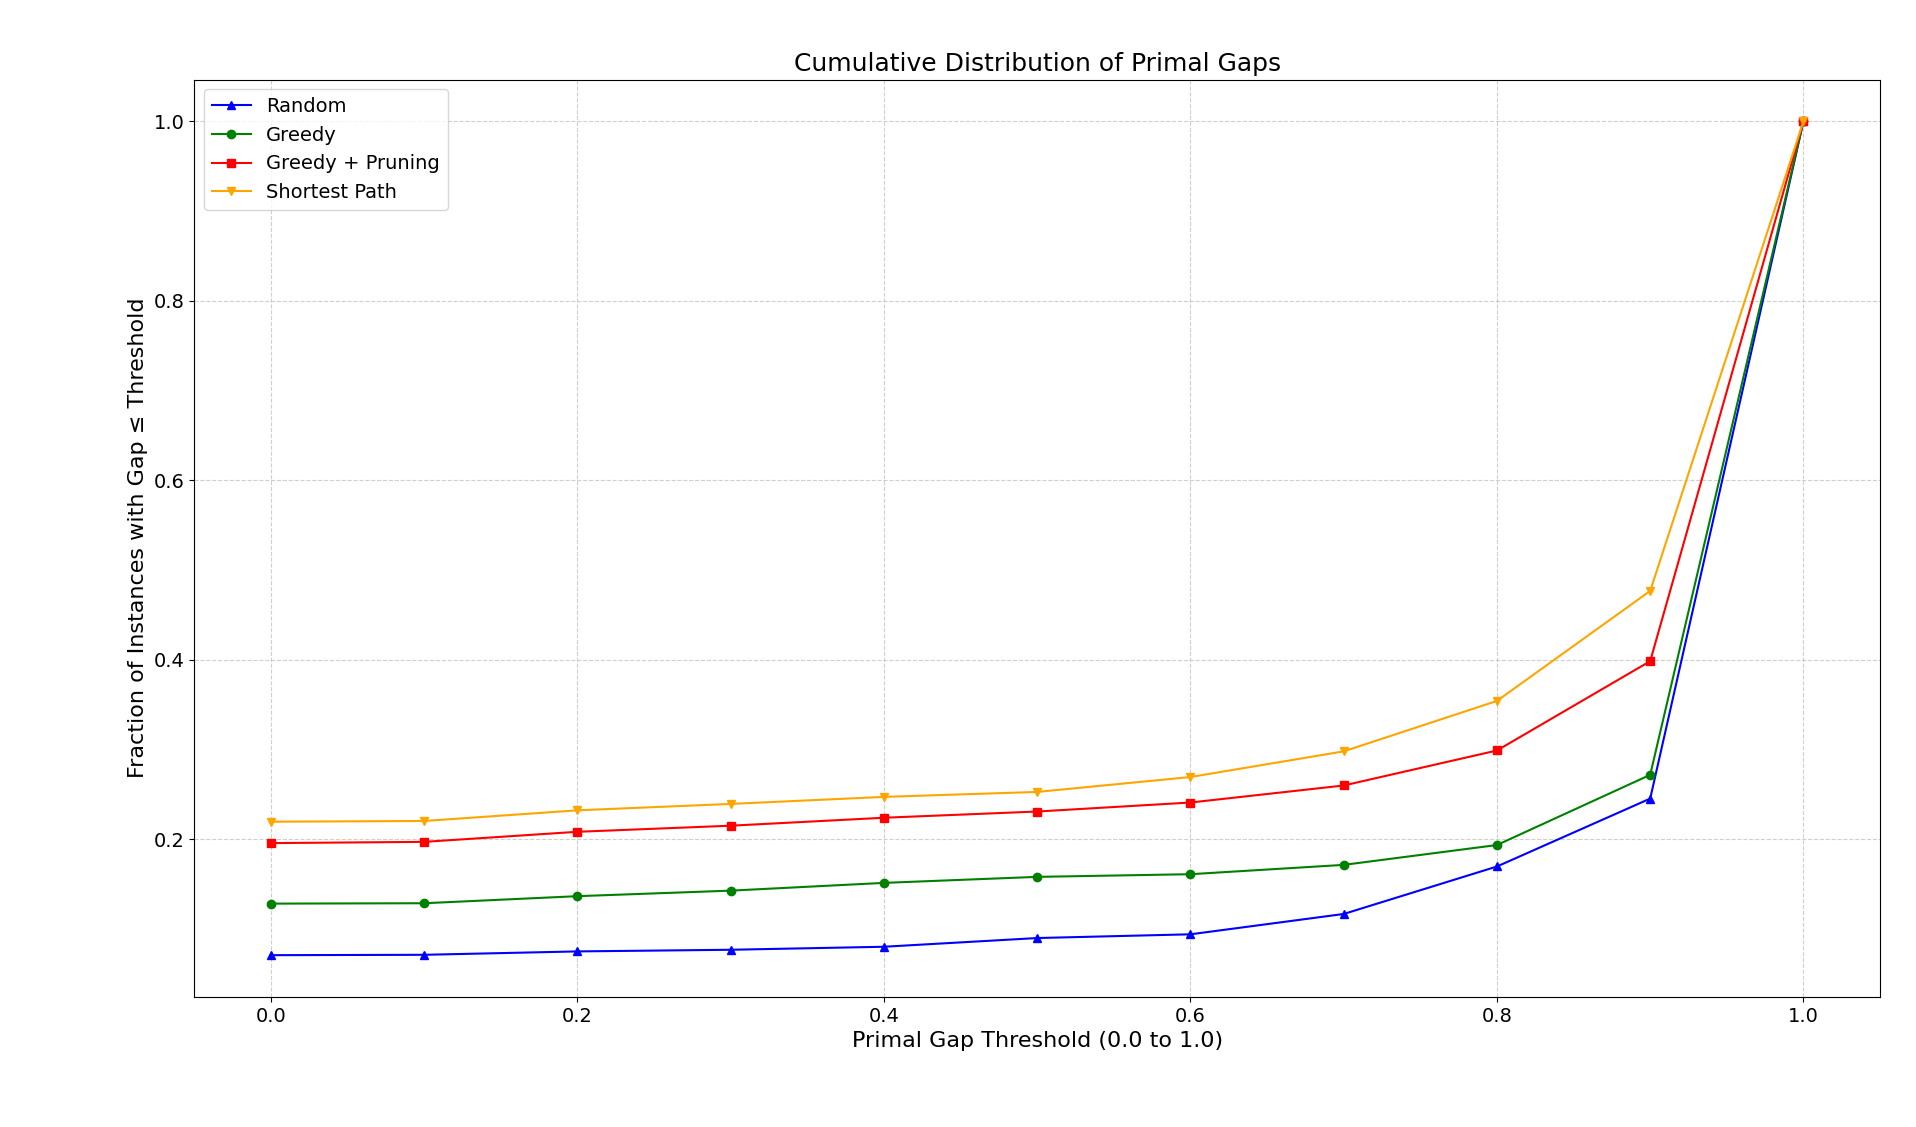
\includegraphics[width=0.75\textwidth]{../thesis/images/algs0124.png}
		\caption{Cumulative distribution plot for Random, Greedy, Greedy + Pruning, and Shortest Path strategies.}
		\label{fig:rgps}
	\end{figure}
\end{frame}

%------------------------------------------------
\section{Refinement Strategies}
%------------------------------------------------

\begin{frame}{Refinement Strategies}
	\begin{itemize}
		\item In the context of Mixed Integer Programming (MIP), there is a technique known as \textit{local branching}
		\item Goal: improve plans produced by heuristics
		\item Attempted approaches:
		      \begin{itemize}
			      \item \textbf{Shortest Path reapplication}
			            \begin{itemize}
				            \item Result: minimal gains
			            \end{itemize}
			      \item \textbf{Uniform Cost Search refinement}
			            \begin{itemize}
				            \item Result: costly, no improvements
			            \end{itemize}

		      \end{itemize}
	\end{itemize}
\end{frame}

%------------------------------------------------
\section{Conclusions}
%------------------------------------------------

\begin{frame}{Conclusions and Future Work}
	\textbf{Conclusions}
	\begin{itemize}
		\item Shortest Path heuristic:
		      \begin{itemize}
			      \item Most effective
			      \item Outperformes baselines in quality and coverage
		      \end{itemize}
		\item Refinement strategies $\rightarrow$ limited benefits
	\end{itemize}
	\textbf{Future Work}
	\begin{itemize}
		\item Explore local branching with optimal external solvers
	\end{itemize}
\end{frame}

%------------------------------------------------

\end{document}
